\documentclass[11pt]{article}

\usepackage{amsmath,amssymb,amsfonts}
\usepackage{graphicx}
\usepackage{pgfplots}
\usepackage{multicol}
\usepackage{enumitem}

\setlength{\topmargin}{-.5in} \setlength{\textheight}{9.25in}
\setlength{\oddsidemargin}{0in} \setlength{\textwidth}{6.8in}


\begin{document}

\Large

\noindent{\bf Name: \hfill Date: \hfill Exam 1 \hfill Precalculus - Hargus}
\medskip\hrule
\vspace{10pt}

\begin{enumerate}

\item (6 points) Write an equation for the linear function $f$ where $f(2) = 5$ and $f(4)=-1$.

\begin{flushright}
$f(x) =$ \rule{4cm}{0.4pt}
\end{flushright}

\item (12 points) Find the domain and the range of the function, and also state the equations for any vertical or horizontal asymptotes.
\begin{enumerate}[itemsep=30pt]
    \item $f(x) = -x^2 + 3$
    \item $f(x) = \sqrt{4-x^2}$
    \item $f(x) = \frac{1}{x-3} + 2$
\end{enumerate}
\vspace{30pt}

\item (6 points) Find the inverse function $f^{-1}(x)$ for the function $f(x) = 7x-4$. \\
\\
\\
\\

\item (12 points) Find the coordinates of the vertex for the following quadratic functions.
\begin{enumerate}[itemsep=60pt]
    \item $f(x) = -2(x-3)^2 + 4$
    \item $f(x) = x^2 - 4x + 7$ \\
\end{enumerate}
\vspace{10pt}

\newpage

\item (6 points) Consider the function $f(x) = -x^3 + 3$. True or false?
\begin{enumerate}[itemsep=20pt]
    \item \rule{1cm}{0.4pt} $f(x)$ has a horizontal asymptote at $y=3$.
    \item \rule{1cm}{0.4pt} $\displaystyle{\lim_{x \to \infty} f(x) = \infty}$
    \item \rule{1cm}{0.4pt} $\displaystyle{\lim_{x \to -\infty} f(x) = \infty}$
\end{enumerate}
\vspace{20pt}

\item (6 points) Let $f(x)=x^3$ and $g(x)=\sqrt[3]{x + 1}$.
\begin{enumerate}[itemsep=20pt]
    \item What is $(f+g)(3)$? \\
    \item What is $(\frac{f}{g})(3)$? \\
    \item What is $(f \circ g)(x)$? What is its domain?
\end{enumerate}
\vspace{50pt}

\item (6 points) Write in the simplified form $a + bi$.
\begin{enumerate}[itemsep=20pt]
    \item $(4-5i) + (2+7i)$ \\
    \item $(1-i)(2+4i)$ \\
    \item $\displaystyle{\frac{i-4}{3i}}$ \\
\end{enumerate}
\vspace{10pt}

\item (6 points) Write the inequality in interval notation. \\ 
\hspace{\parindent} $|x-4| \geq 1$.

\newpage

\item (8 points) Use the Rational Zeros Theorem to list all \textbf{possible} rational zeros for the function $f(x) = 3x^3 + x^2 + 2$. Then, plug in to find which ones are \textbf{actual} zeros.

\vspace{20pt}

\begin{flushright}
Possible rational zeros: $x=$ \rule{4cm}{0.4pt} \\
\vspace{20pt}
Actual rational zeros: $x=$ \rule{4cm}{0.4pt}
\end{flushright}

\vspace{20pt}

\item (8 points) Use synthetic division to divide the following (Write the final answer in \textbf{fraction form}).

\vspace{10pt}
$\displaystyle{\frac{2x^3 - 5x^2 + 3x + 7}{x-2}}$
\vspace{60pt}

\item (6 points) Find the zeroes of the following functions. 
\begin{enumerate}[itemsep=10pt]
    \item $f(x) = 2x^2 + x - 1$
    \vspace{60pt}
    \begin{flushright}
    $x=$ \rule{4cm}{0.4pt}
    \end{flushright}

    \item $f(x) = x(x-2)(x-3)^2$
    \vspace{60pt}
    \begin{flushright}
    $x=$ \rule{4cm}{0.4pt}
    \end{flushright}
\end{enumerate}


\newpage

\item (6 points) The graph of $f(x)=-x^3$ is drawn below. Draw $g(x)=(x-3)^3-5$. (Note: pay attention to the different scales on the axes)
\vspace{4pt}
\begin{center}
\begin{tikzpicture}
\begin{axis}[ xlabel={$x$}, ylabel={$y$}
  ,axis lines=middle
  ,samples=1000, grid, thick
  ,domain=-10:10
  ,legend pos=outer north east
  ,xmin=-5, xmax=5,
  ,ymin=-10, ymax=10
  ]
\addplot+[no marks] {-x^3};
\addlegendentry{$f(x)$}
\end{axis}
\end{tikzpicture}
\end{center}

\item (6 points) The graph of $f(x)$ is drawn below. Draw the graph of $f^{-1}(x)$.
\vspace{10pt}
\begin{center}
\begin{tikzpicture}
\begin{axis}[ xlabel={$x$}, ylabel={$y$}
  ,axis lines=middle
  ,samples=1000, grid, thick
  ,domain=-10:10
  ,axis equal
  ,legend pos=outer north east
  ,xmin=-5, xmax=5,
  ,ymin=-5, ymax=5
  ]
\addplot+[no marks] {(x+3)^2*(x-3)/20};
\addlegendentry{$f(x)$}
\end{axis}
\end{tikzpicture}
\end{center}

\item (6 points) Please sketch the graph of $f(x) = (x+1)(x-2)(x-3)$.
\vspace{10pt}
\begin{center}
\begin{tikzpicture}
\begin{axis}[ xlabel={$x$}, ylabel={$y$}
  ,axis lines=middle
  ,samples=1000, grid, thick
  ,domain=-10:10
  ,axis equal
  ,legend pos=outer north east
  ,xmin=-6, xmax=6,
  ,ymin=-5, ymax=5
  ];
% \addplot+[no marks] {(x+3)^2*(x-3)/20};
\end{axis}
\end{tikzpicture}
\end{center}

\end{enumerate}

\end{document} 